\section{Sending Authenticated Encrypted Payload To Ditto}

This section demonstrates the proof of concept securing the communication between the IoT device and the Digital Twin (Ditto). 

Figure \ref{fig:log-mon} depicts a snapshot captured from the serial monitor output of the board (device) utilizing PlatformIO (embedded development framework). The image showcases the device transmitting an encrypted payload to the 'ut-sensors' topic while including additional data labeled as 'tid' to uniquely identify the device. In Figure \ref{fig:wireshark}, a captured packet during the communication is displayed. Upon observation, it becomes evident that the topic being utilized is 'ut-sensors', and the message section of the MQTT protocol header contains the device identifier along with the encrypted payload.


\begin{figure}[H]
    \caption{Serial Monitor of ESP32 Board and Wireshark Capturing Communication Between The Device and Ditto(DT)}
    \begin{subfigure}[c]{1\linewidth}
        \centering
        \caption{Log Output of ESP32 Device Using Serial Monitor}
        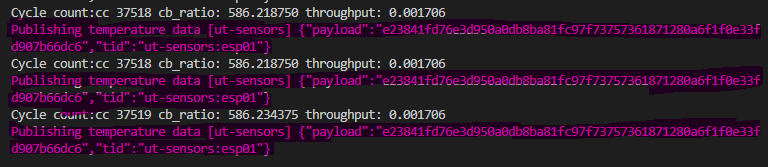
\includegraphics[width=\linewidth]{images/fp/serialport.png}
        \label{fig:log-mon}
     \end{subfigure}    

    \begin{subfigure}[c]{1\linewidth}
        \centering
        \caption{Wireshark Captured MQTT Communication From IoT to Ditto}
        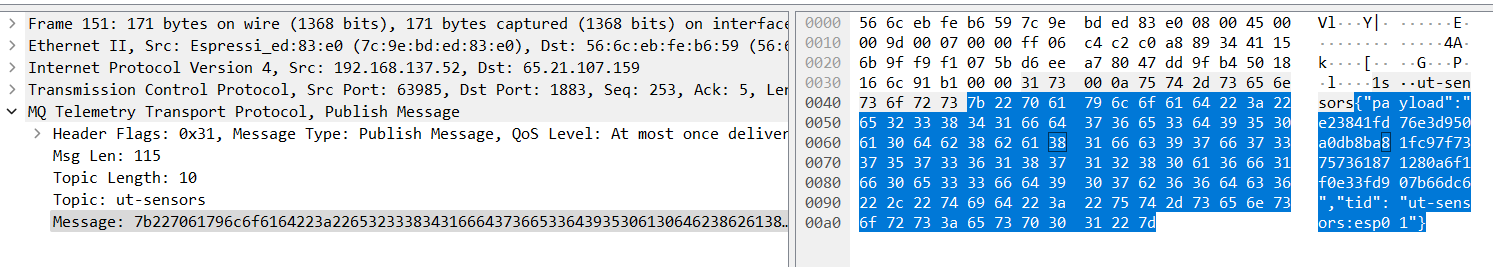
\includegraphics[width=\linewidth]{images/fp/wireshark.png}
        \label{fig:wireshark}
    \end{subfigure}
\end{figure}

The MQTT broker, hosted on the same server  with Ditto, acts as a proxy, facilitating the transmission of authenticated and encrypted payloads through a publish-subscribe model. Once the MQTT broker receives a payload, it  notifies Ditto of the new message it has subscribed to. Ditto then retrieves the payload, decrypts it, and maps it into a Ditto protocol message, which is subsequently stored in a database.

To simulate the life cycle of a Digital Twin, we have developed a small web application that models the temperature and humidity features of an ESP32 sensor. The application utilizes JavaScript to retrieve these values through a stream of emissions using server-side events (SSE). Moreover, to send commands or messages to the server, we employ the HTTP POST API of Ditto. By subscribing to the command event associated with a specific topic, any device can consume the message and execute the corresponding action. This activity effectively simulates the communication between the digital twin and the actuators. Conversely, the communication from the IoT device to the Digital Twin serves the purpose of collecting telemetry data from the operational environment.

Figure \ref{fig:ditto-log} illustrates the WebUI of Ditto, which is included by default in the code base. This web portal serves as a portal offering device, policy, and connection management functionalities. Additionally, Figure \ref{fig:appdt} provides an overview of an application layer built on the Digital Twin concept. The attributes displayed on the upper part of the image represent the name and type of the simulated device. The gauges visually represent the received device features, while the bottom right section presents textual information associated with the device.
 
\begin{figure}[H]
    \caption{Ditto and Webapp Toward Simulating Digital Twin}
    \label{fig:ditto-app}
    \begin{subfigure}[c]{1\linewidth}
        \caption{A Data Log Viewed from Ditto Platform}
        \centering
        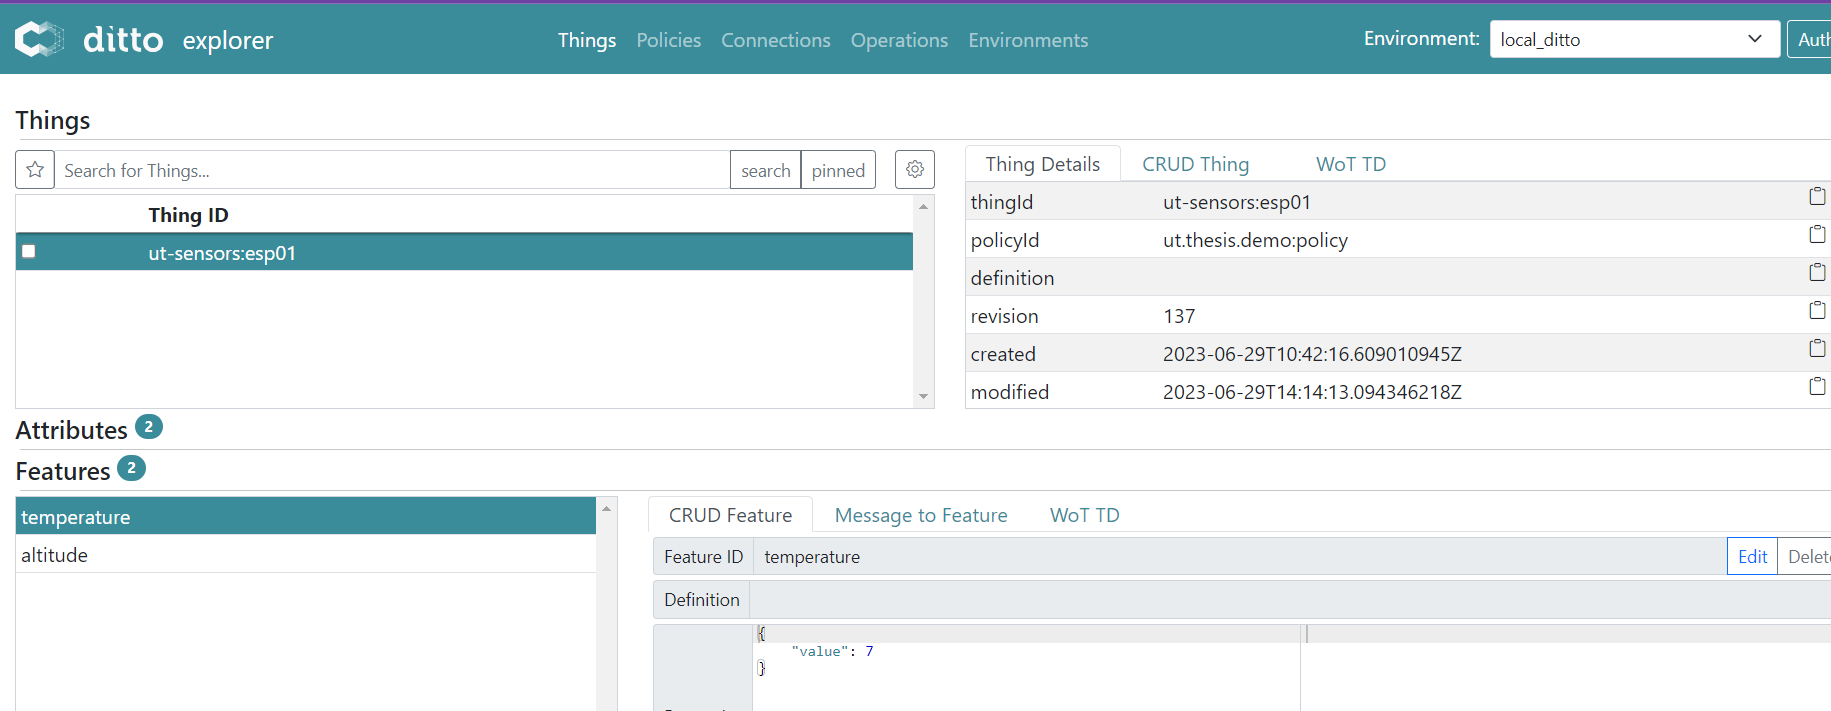
\includegraphics[width=\linewidth]{images/fp/ditto-log.png}
        \label{fig:ditto-log}
    \end{subfigure}
    
    \begin{subfigure}[c]{1\linewidth}
        \centering
        \caption{Web Application For Modeling Temperature and Humidity of ESP32}
        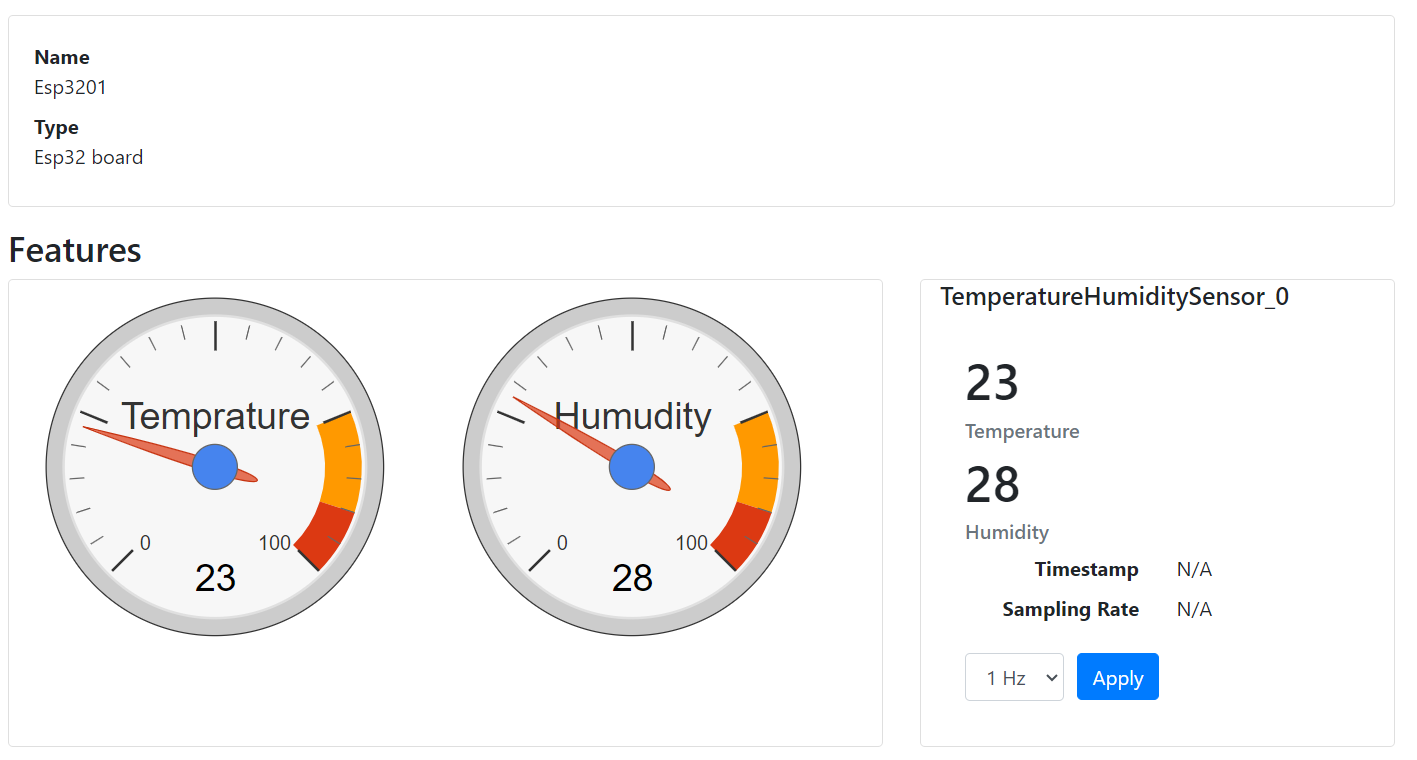
\includegraphics[width=\linewidth]{images/fp/appgauge.png}
        \label{fig:appdt}
     \end{subfigure}    
\end{figure}